\documentclass{beamer}

%Setting theme of beamer
\mode<presentation>{

% The Beamer class comes with a number of default slide themes
% which change the colors and layouts of slides. Below this is a list
% of all the themes, uncomment each in turn to see what they look like.

%\usetheme{default}
%\usetheme{AnnArbor}
%\usetheme{Antibes}
%\usetheme{Bergen}
%\usetheme{Berkeley}
%\usetheme{Berlin}
%\usetheme{Boadilla}
%\usetheme{CambridgeUS}
%\usetheme{Copenhagen}
%\usetheme{Darmstadt}
%\usetheme{Dresden}
%\usetheme{Frankfurt}
%\usetheme{Goettingen}
%\usetheme{Hannover}
%\usetheme{Ilmenau}
%\usetheme{JuanLesPins}
%\usetheme{Luebeck}
\usetheme{Madrid}
%\usetheme{Malmoe}
%\usetheme{Marburg}
%\usetheme{Montpellier}
%\usetheme{PaloAlto}
%\usetheme{Pittsburgh}
%\usetheme{Rochester}
%\usetheme{Singapore}
%\usetheme{Szeged}
%\usetheme{Warsaw}

% As well as themes, the Beamer class has a number of color themes
% for any slide theme. Uncomment each of these in turn to see how it
% changes the colors of your current slide theme.

\usecolortheme{default}
%\usecolortheme{albatross}
%\usecolortheme{beaver}
%\usecolortheme{beetle}
%\usecolortheme{crane}
%\usecolortheme{dolphin}
%\usecolortheme{dove}
%\usecolortheme{fly}
%\usecolortheme{lily}
%\usecolortheme{orchid}
%\usecolortheme{rose}
%\usecolortheme{seagull}
%\usecolortheme{seahorse}
%\usecolortheme{whale}
%\usecolortheme{wolverine}

%\setbeamertemplate{footline} % To remove the footer line in all slides uncomment this line
%\setbeamertemplate{footline}[frame number] % To replace the footer line in all slides with a simple slide count uncomment this line

%\setbeamertemplate{navigation symbols}{} % To remove the navigation symbols from the bottom of all slides uncomment this line

\setbeamercovered{transparent}

%\usefonttheme{serif}

%\newcommand*\oldmacro{}%
%\let\oldmacro\insertshorttitle%
%\renewcommand*\insertshorttitle{%
  %\oldmacro\hfill%
  %\insertframenumber\,/\,\inserttotalframenumber}

\setbeamertemplate{caption}[numbered]
\setbeamercolor{caption name}{fg=structure!70!black}
}


%Import other required packages, e.g. 'ctex'
\usepackage[T1]{fontenc}        % Encoding
\usepackage[utf8]{inputenc}     % Encoding
\usepackage{multicol}
\usepackage{ctex}               % Support for zh_cn
\usepackage{amsmath}            % Allows math
%\usepackage{newtxtext,newtxmath}
\usepackage{mathptmx}
\usepackage{graphicx}           % Allows including images
\usepackage{wrapfig}            % Images placement require
\usepackage{float}              % Images float
\usepackage{subfigure}          % subplot support
\usepackage{booktabs}           % Allows the use of \toprule, \midrule and \bottomrule in tables
\usepackage{tcolorbox}          % Allows color table
\usepackage{multirow}           % Allows multiple row in table
\usepackage{enumerate}          % Allows enumerate

%\usepackage[linesnumbered,ruled]{algorithm2e} % Allows algorithm
\usepackage{algpseudocode}
%\renewcommand{\algorithmcfname}{算法} % Change 'Algorithm x' to '算法 x'

%-----------------------------------------------------------
%This block of code defines the information to appear in the
%Title page
\title[Master Thesis Defense]
{基于容器的负载预测模型\\
与能耗优化调度策略研究}

\author[ZeTao Wang]
{答辩人:~王泽涛\inst{1} \and 导师:~林伟伟\inst{2}}

\institute[SCUT]
{
    \inst{1}
    华南理工大学\ 计算机科学与工程学院
    \and
    \inst{2}
    华南理工大学\ 计算机科学与工程学院
}

\logo{

\includegraphics[scale=0.2]{figures/logo.jpg}
}

\date[June. 2019]
{2019年6月}
%End of title page configuration
%-----------------------------------------------------------



%-----------------------------------------------------------
%The next block of commands puts the table of contents at the
%beginning of each section and highlights the current section:

\AtBeginSection[]
{
  \begin{frame}
    \frametitle{目录}
    \tableofcontents[currentsection]
  \end{frame}
}
%-----------------------------------------------------------


\begin{document}

%Title of the document
%This next statement create title page
\frame{\titlepage}

%---------------------------------------------------------
%This block of code is for the table of contents after
%the title page
\begin{frame}
\frametitle{目录}
\tableofcontents[hideothersubsections]
\end{frame}
%---------------------------------------------------------

%Background
%Title of section
\section{问题背景}

\begin{frame}
\frametitle{问题背景}
\begin{itemize}
    \item<1-> 虚拟机和容器
    \begin{itemize}
        \item<1-> 虚拟机:Hypervisor
        \item<1-> 容器:Namespace和CGgroups
    \end{itemize}
    \item<2-> 云计算运行模式:IaaS,PaaS和SaaS转变到CaaS
    \begin{itemize}
        \item<2-> \color{green}{容器简单部署和快速可用}
        \item<2-> \color{gray}{\sout{安全问题}}
        \item<2-> \color{gray}{\sout{资源抢占}}
        \item<2-> \color{blue}{\checkmark CaaS性能损耗低}
    \end{itemize}
    \item<3-> 能耗优化与绿色计算
\end{itemize}

\begin{figure}[htb]
\visible<1->{
    \centering
    \begin{minipage}{130pt}
    \centering
    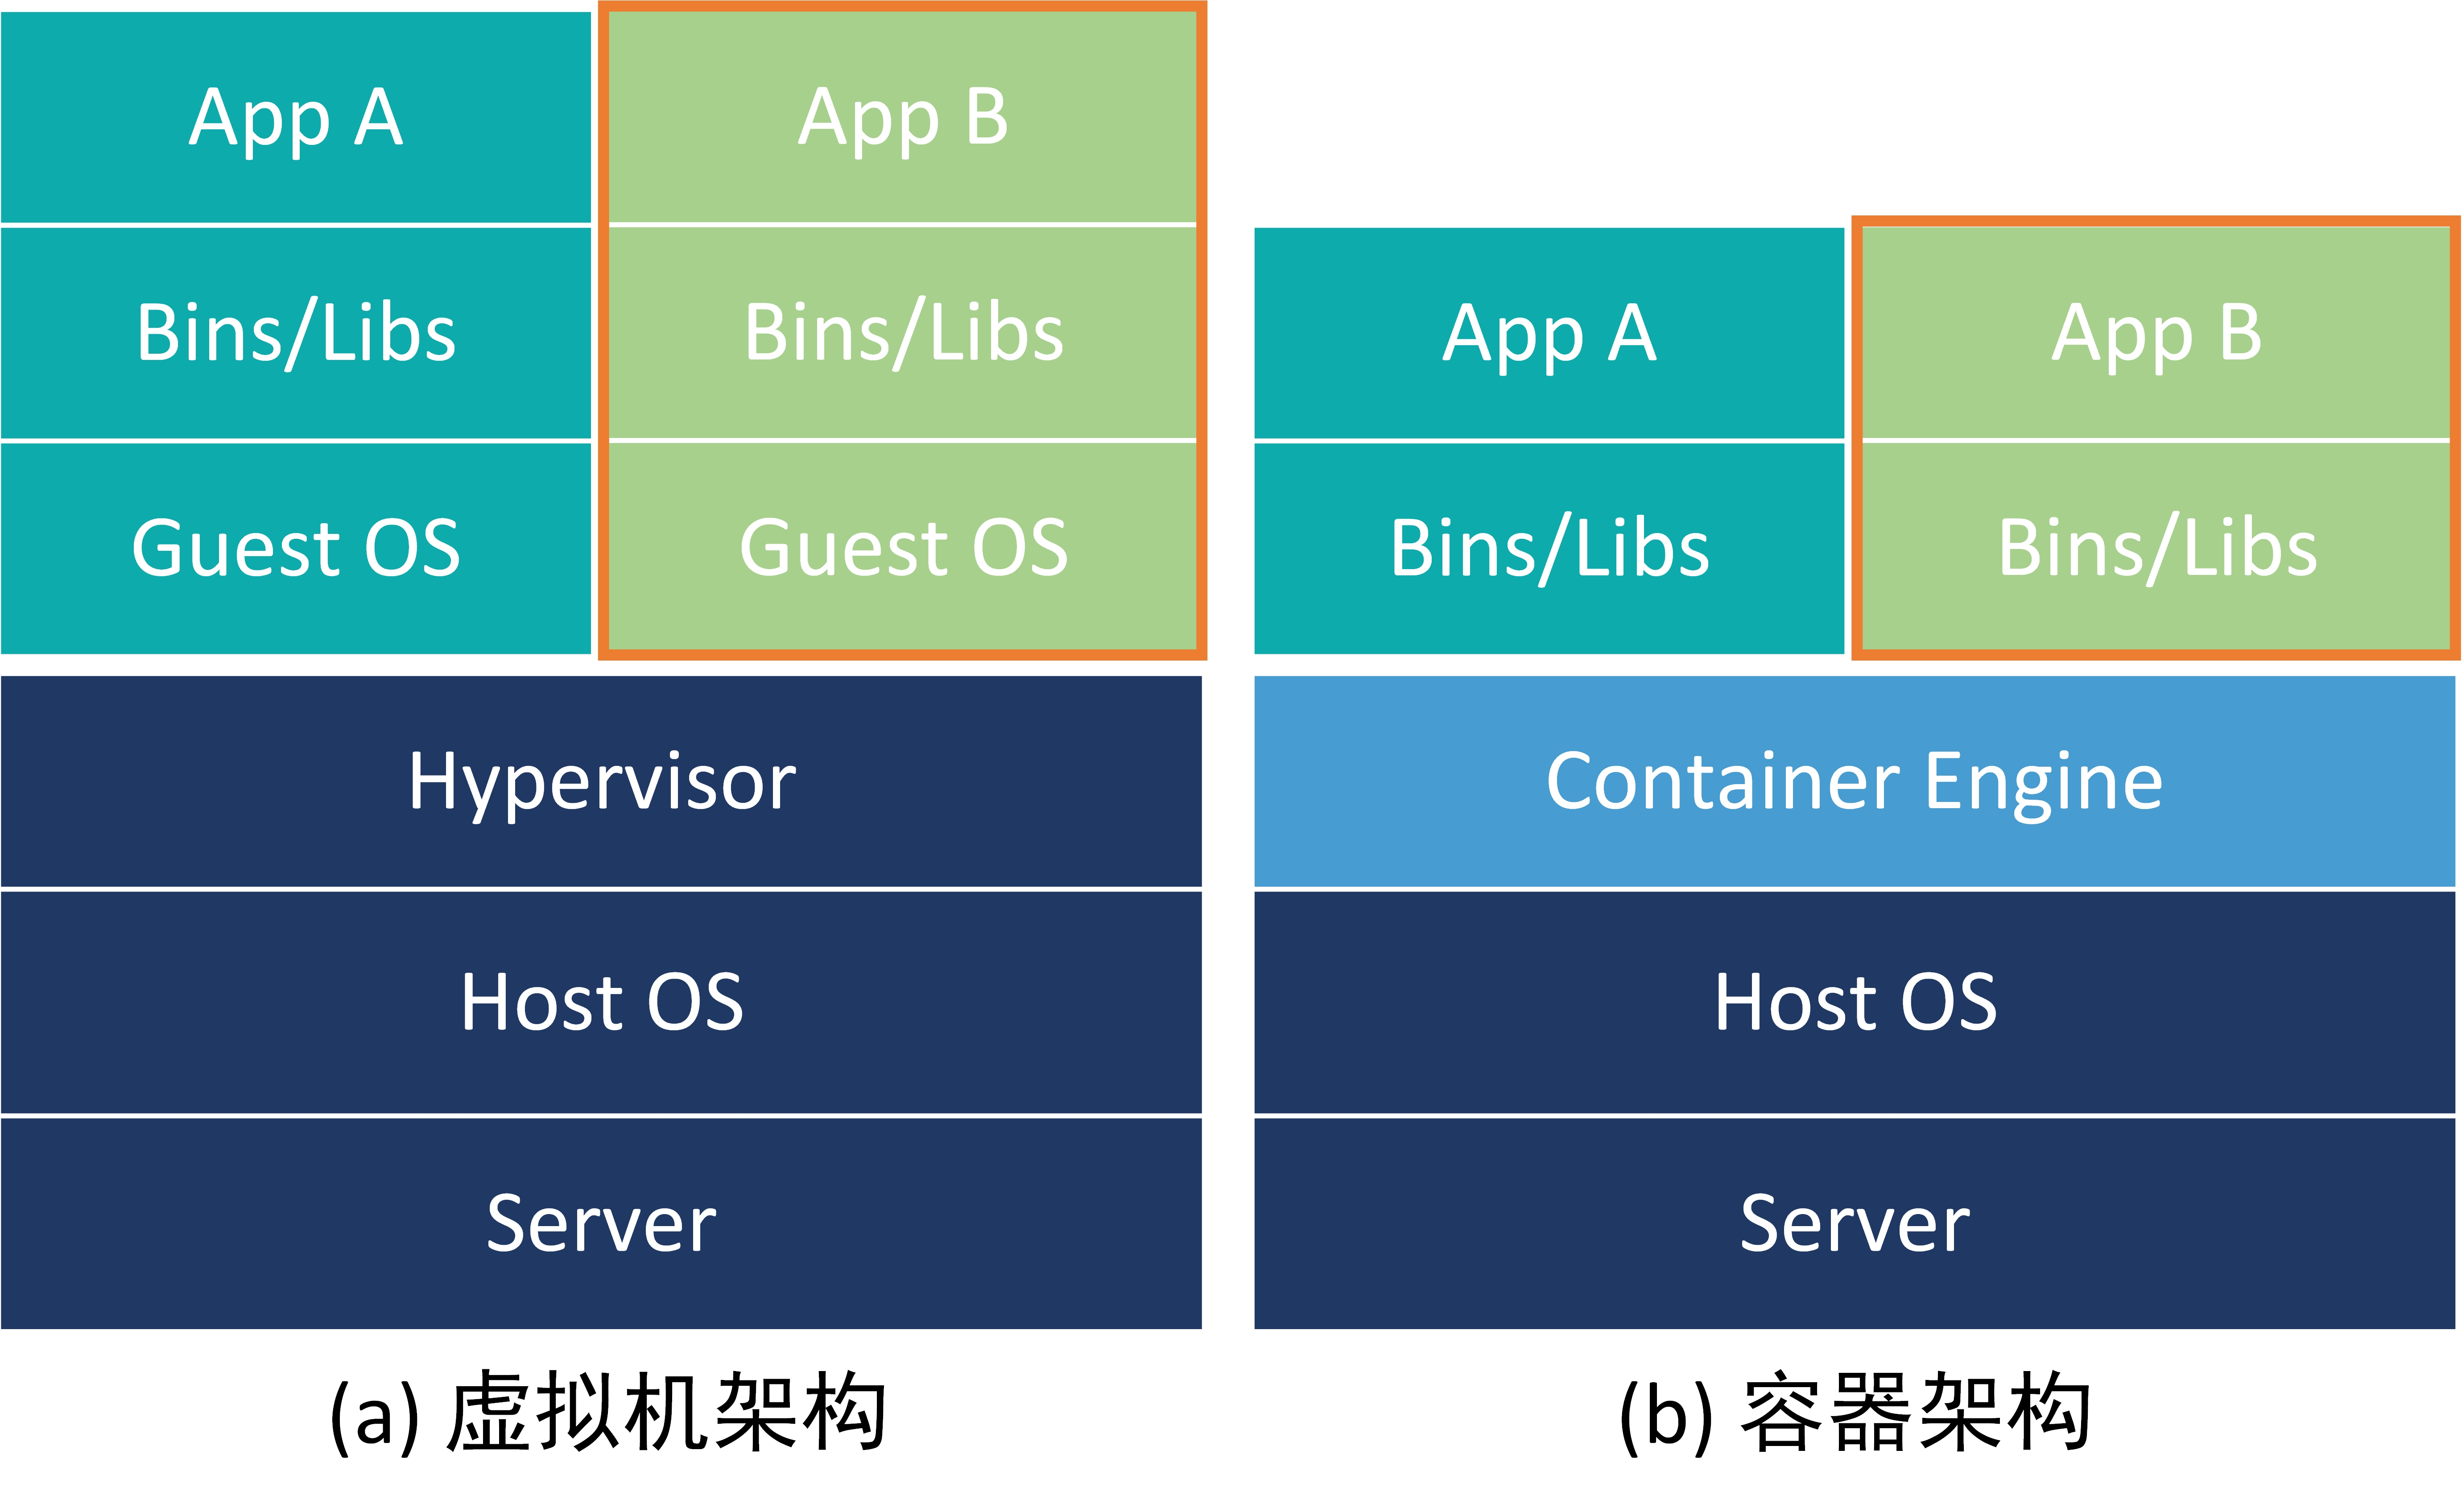
\includegraphics[scale=0.41]{figures/fig1_vm_vs_container.jpg}
    \caption{VM vs Container}
    \label{fig:fig1}
    \end{minipage}
}
\hspace{20pt}%
\visible<2->{
    \begin{minipage}{130pt}
    \centering
    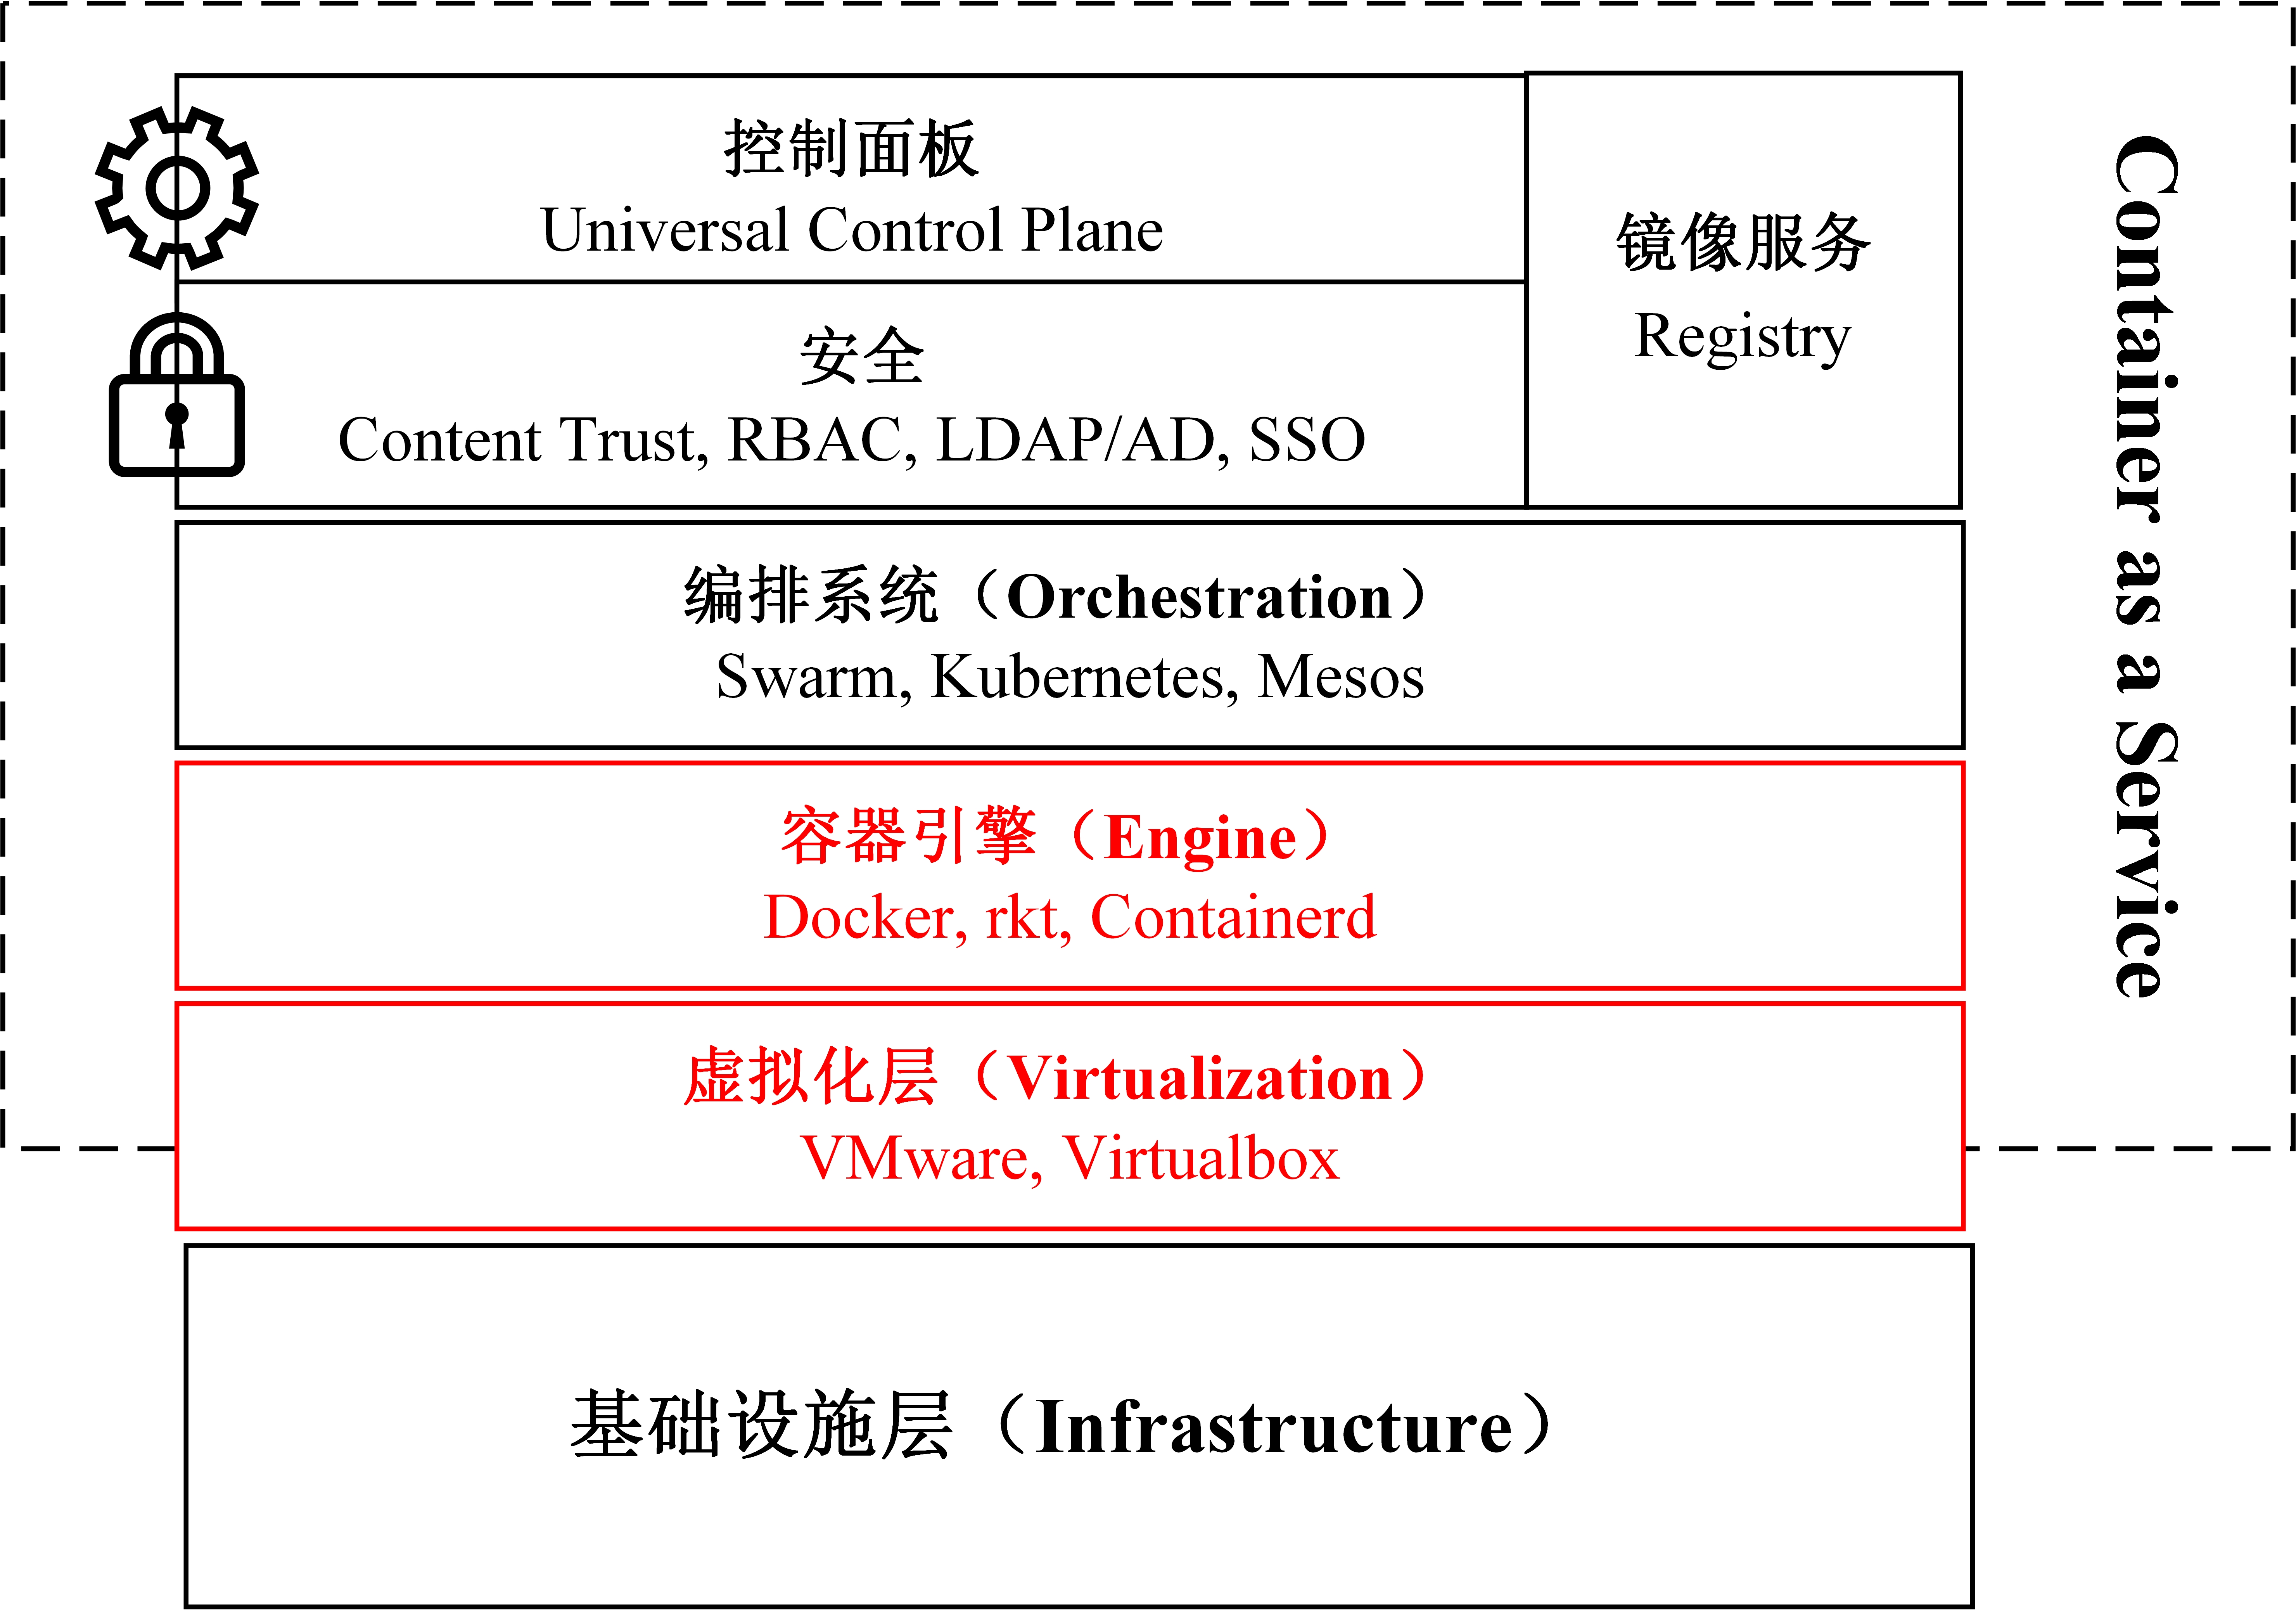
\includegraphics[scale=0.3]{figures/fig2_caas.jpg}
    \caption{CaaS架构示意图}
    \label{fig:fig2}
    \end{minipage}
}
\end{figure}

\end{frame}


%Motivation
%Title of section
\section{研究动机}

\subsection{主要目标}

\begin{frame}
\frametitle{研究动机}
\framesubtitle{主要目标}
\begin{block}{解决CaaS模式下云数据中心的能耗优化问题}
    \begin{itemize}
        \item 负载监控机制:负载与能耗紧密相关
        \begin{itemize}
            \item 实时性
            \item 准确性
            \item 易扩展性
        \end{itemize}
        \item 基于负载状态容器调度策略
        \begin{itemize}
            \item 保证云服务QoS(Quality of Service)
            \item 降低整体能耗
        \end{itemize}
    \end{itemize}
\end{block}
\end{frame}

\subsection{负载监控}

\begin{frame}
\frametitle{研究动机}
\framesubtitle{负载监控}
容器负载监控机制对云数据中心\textbf{\alert{资源配置和调度决策}}有较大影响

\begin{block}{负载监控机制}
\begin{itemize}
    \item<1-> 基于负载采集程序:负载变化频繁、异构网络环境导致滞后性
    \item<2-> 负载预测模型:主动进行资源配置和容器调度
\end{itemize}
\end{block}
\begin{figure}[htb]
\centering
    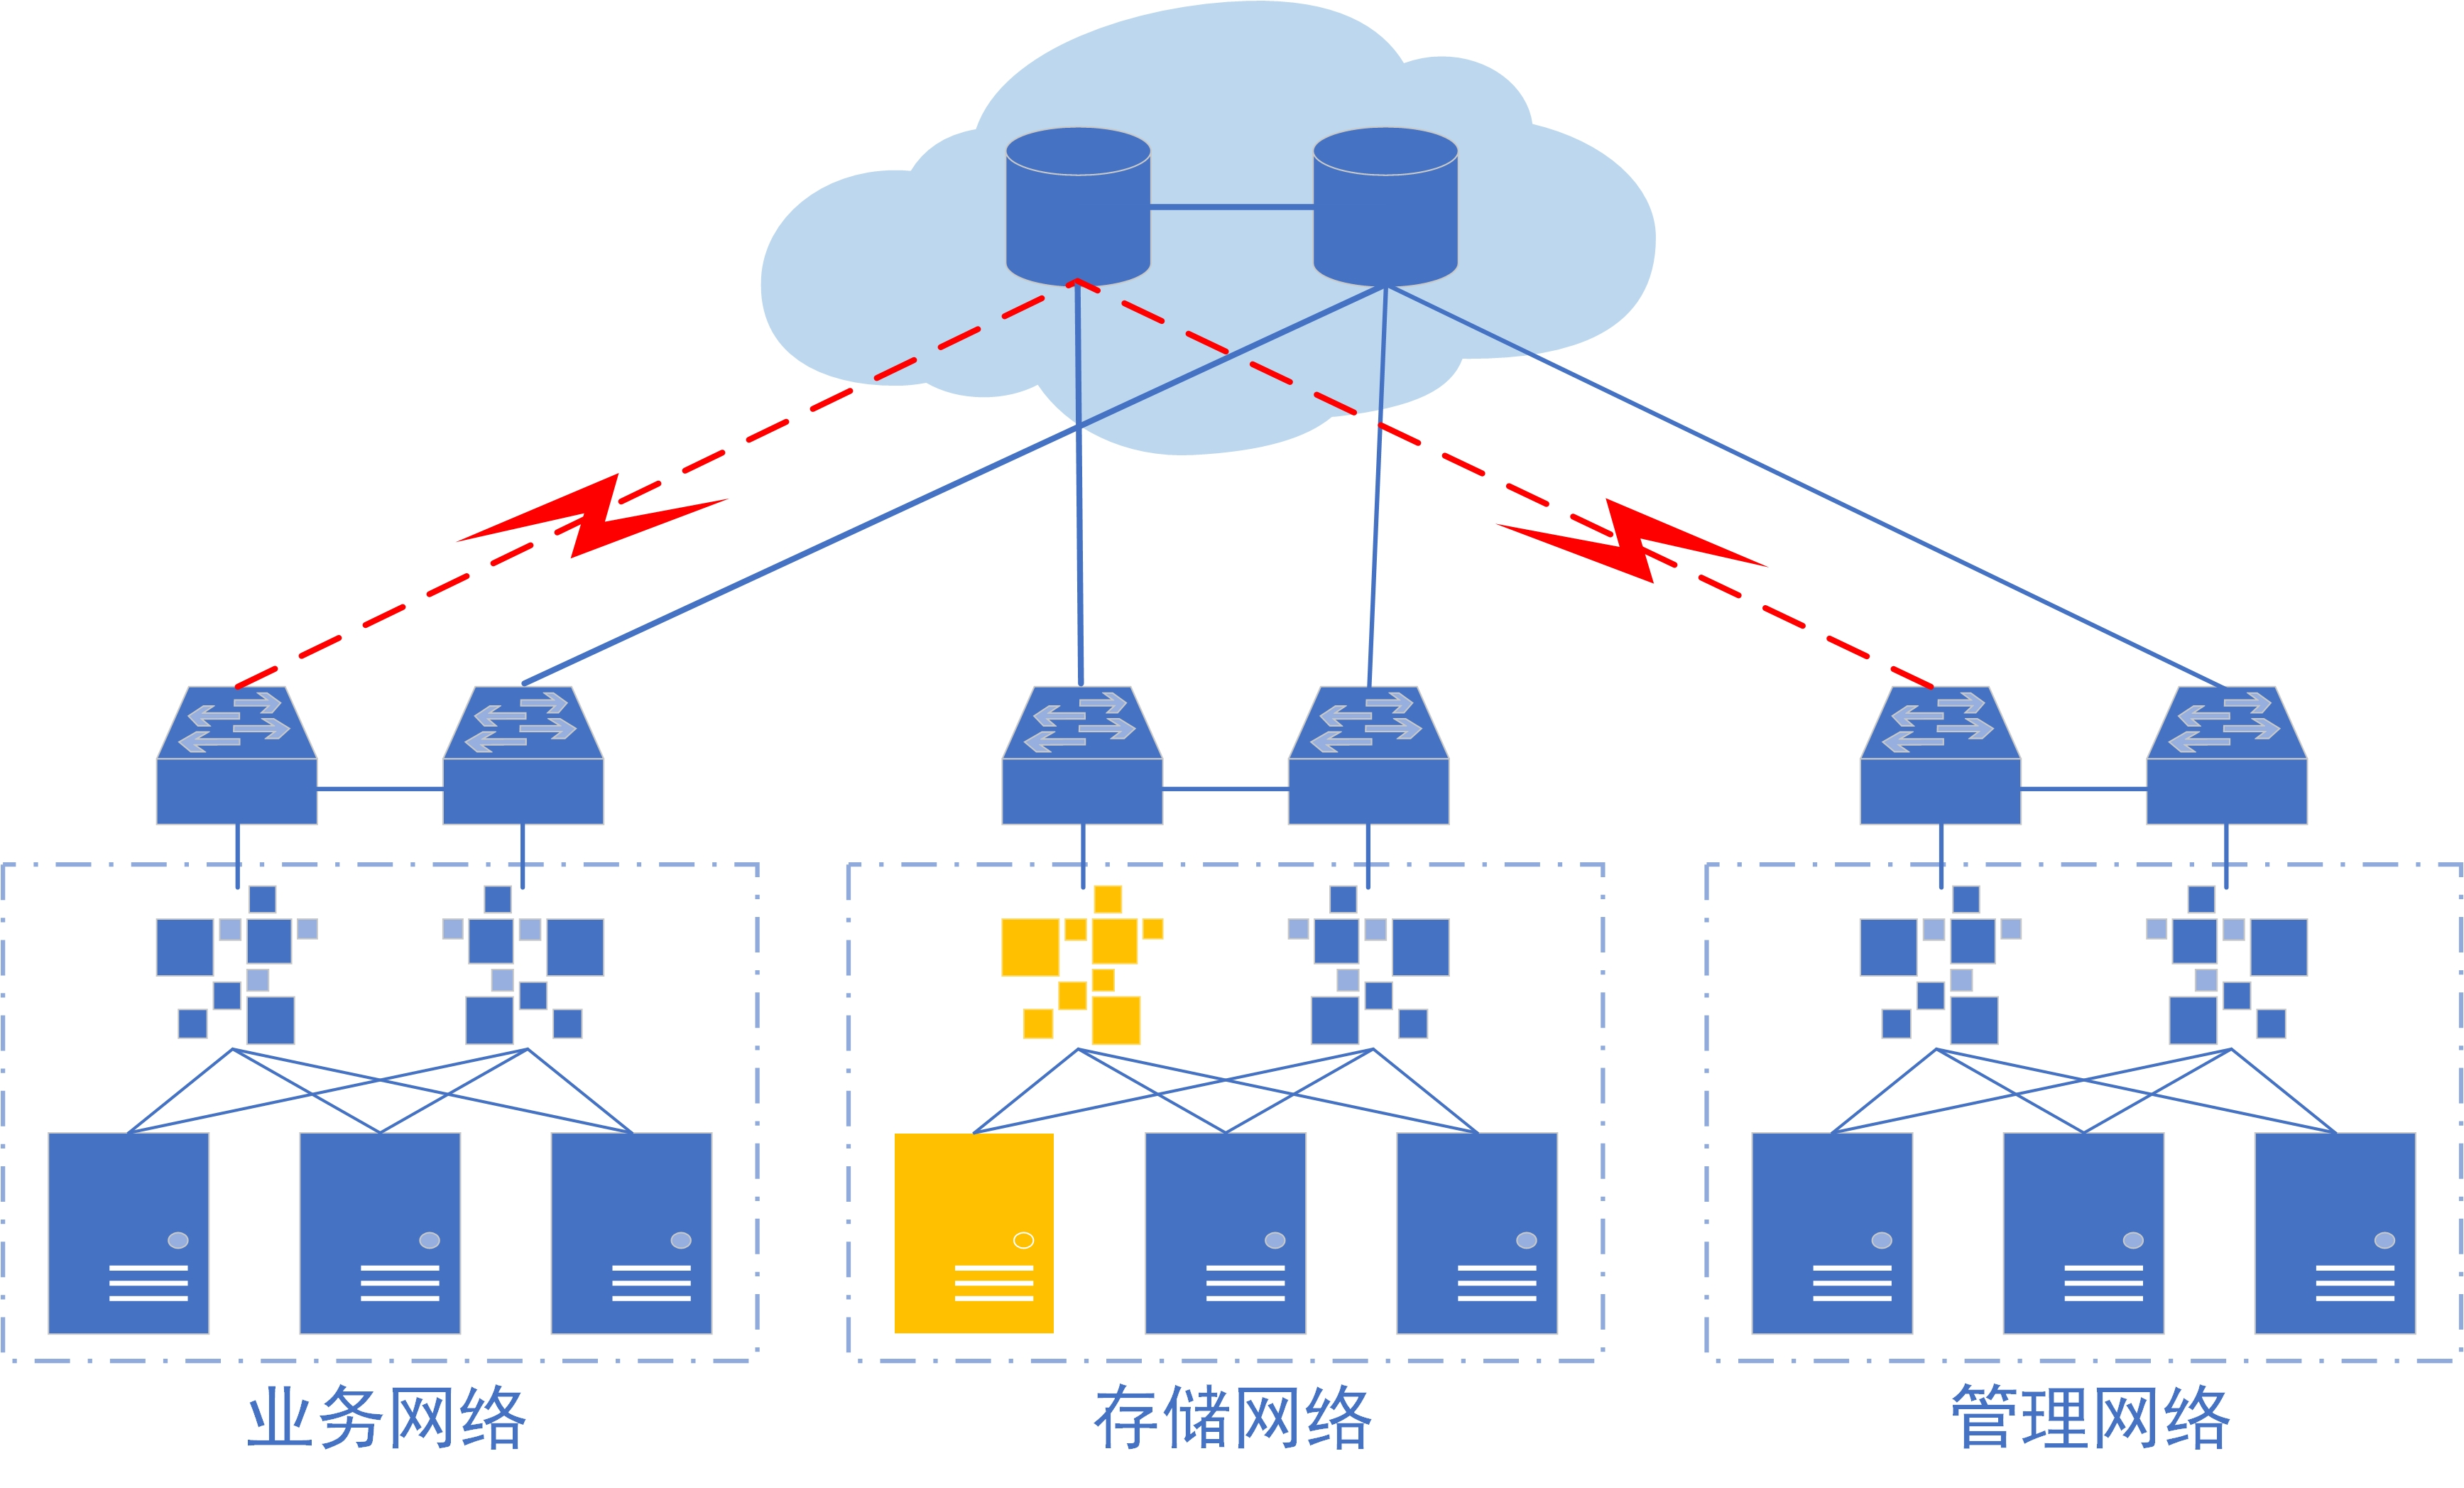
\includegraphics[scale=0.41]{figures/fig3_mmn.jpg}
    \caption{基于负载采集程序的监控网络}
    \label{fig:fig3}
\end{figure}
\end{frame}

\begin{frame}
\frametitle{研究动机}
\framesubtitle{负载监控}
\begin{block}{负载预测模型}
\begin{itemize}
    \item<1-1> 单值预测模型:预测特定值
    \begin{itemize}
        \item<1-1> \textbf{误差敏感} $\Rightarrow$ \textbf{决策失效}
        \item<1-1> \textbf{鲁棒性差} $\Rightarrow$ \textbf{决策过度}
    \end{itemize}
    \item<2-2> 区间预测模型:预测取值区间(置信度$\alpha=0.9$)
\end{itemize}
\end{block}

\vspace*{-0.7cm}
\visible<1>{
\begin{columns}
\begin{column}{0.6\textwidth}
    \centering
    \begin{table}[hftb]
    \centering
    \resizebox{\textwidth}{!}{%
        \begin{tabular}{ccl}
            \toprule
            \textbf{类型} & \textbf{模型名称} & \textbf{简述}\\
            \midrule
            \multirow{4}{*}{统计学模型} & ARIMA & 差分自回归移动平均\\
            ~ & Kalman滤波 & 基于递推演进和观测值对预测结果进行演进\\
            ~ & 排队论模型 & 基于在线作业请求和系统阻塞情况进行预测\\
            ~ & 灰色模型 & 模型新陈代谢过程,进行中长期预测\\
            \midrule
            \multirow{4}{*}{机器学习模型} & RNN & 递归神经网络预测\\
            ~ & BPNN & 原始信息前向传播,误差信息后向传播\\
            ~ & LSTM & 长短期记忆网络\\
            ~ & 混合模型 & 基于c-means聚类和模糊(Fuzzy)神经网络\\
            \bottomrule
        \end{tabular}
    }
    \caption{单值预测模型}
    \end{table}
\end{column}
\begin{column}{0.3\textwidth}
\centering
\begin{figure}[htb]
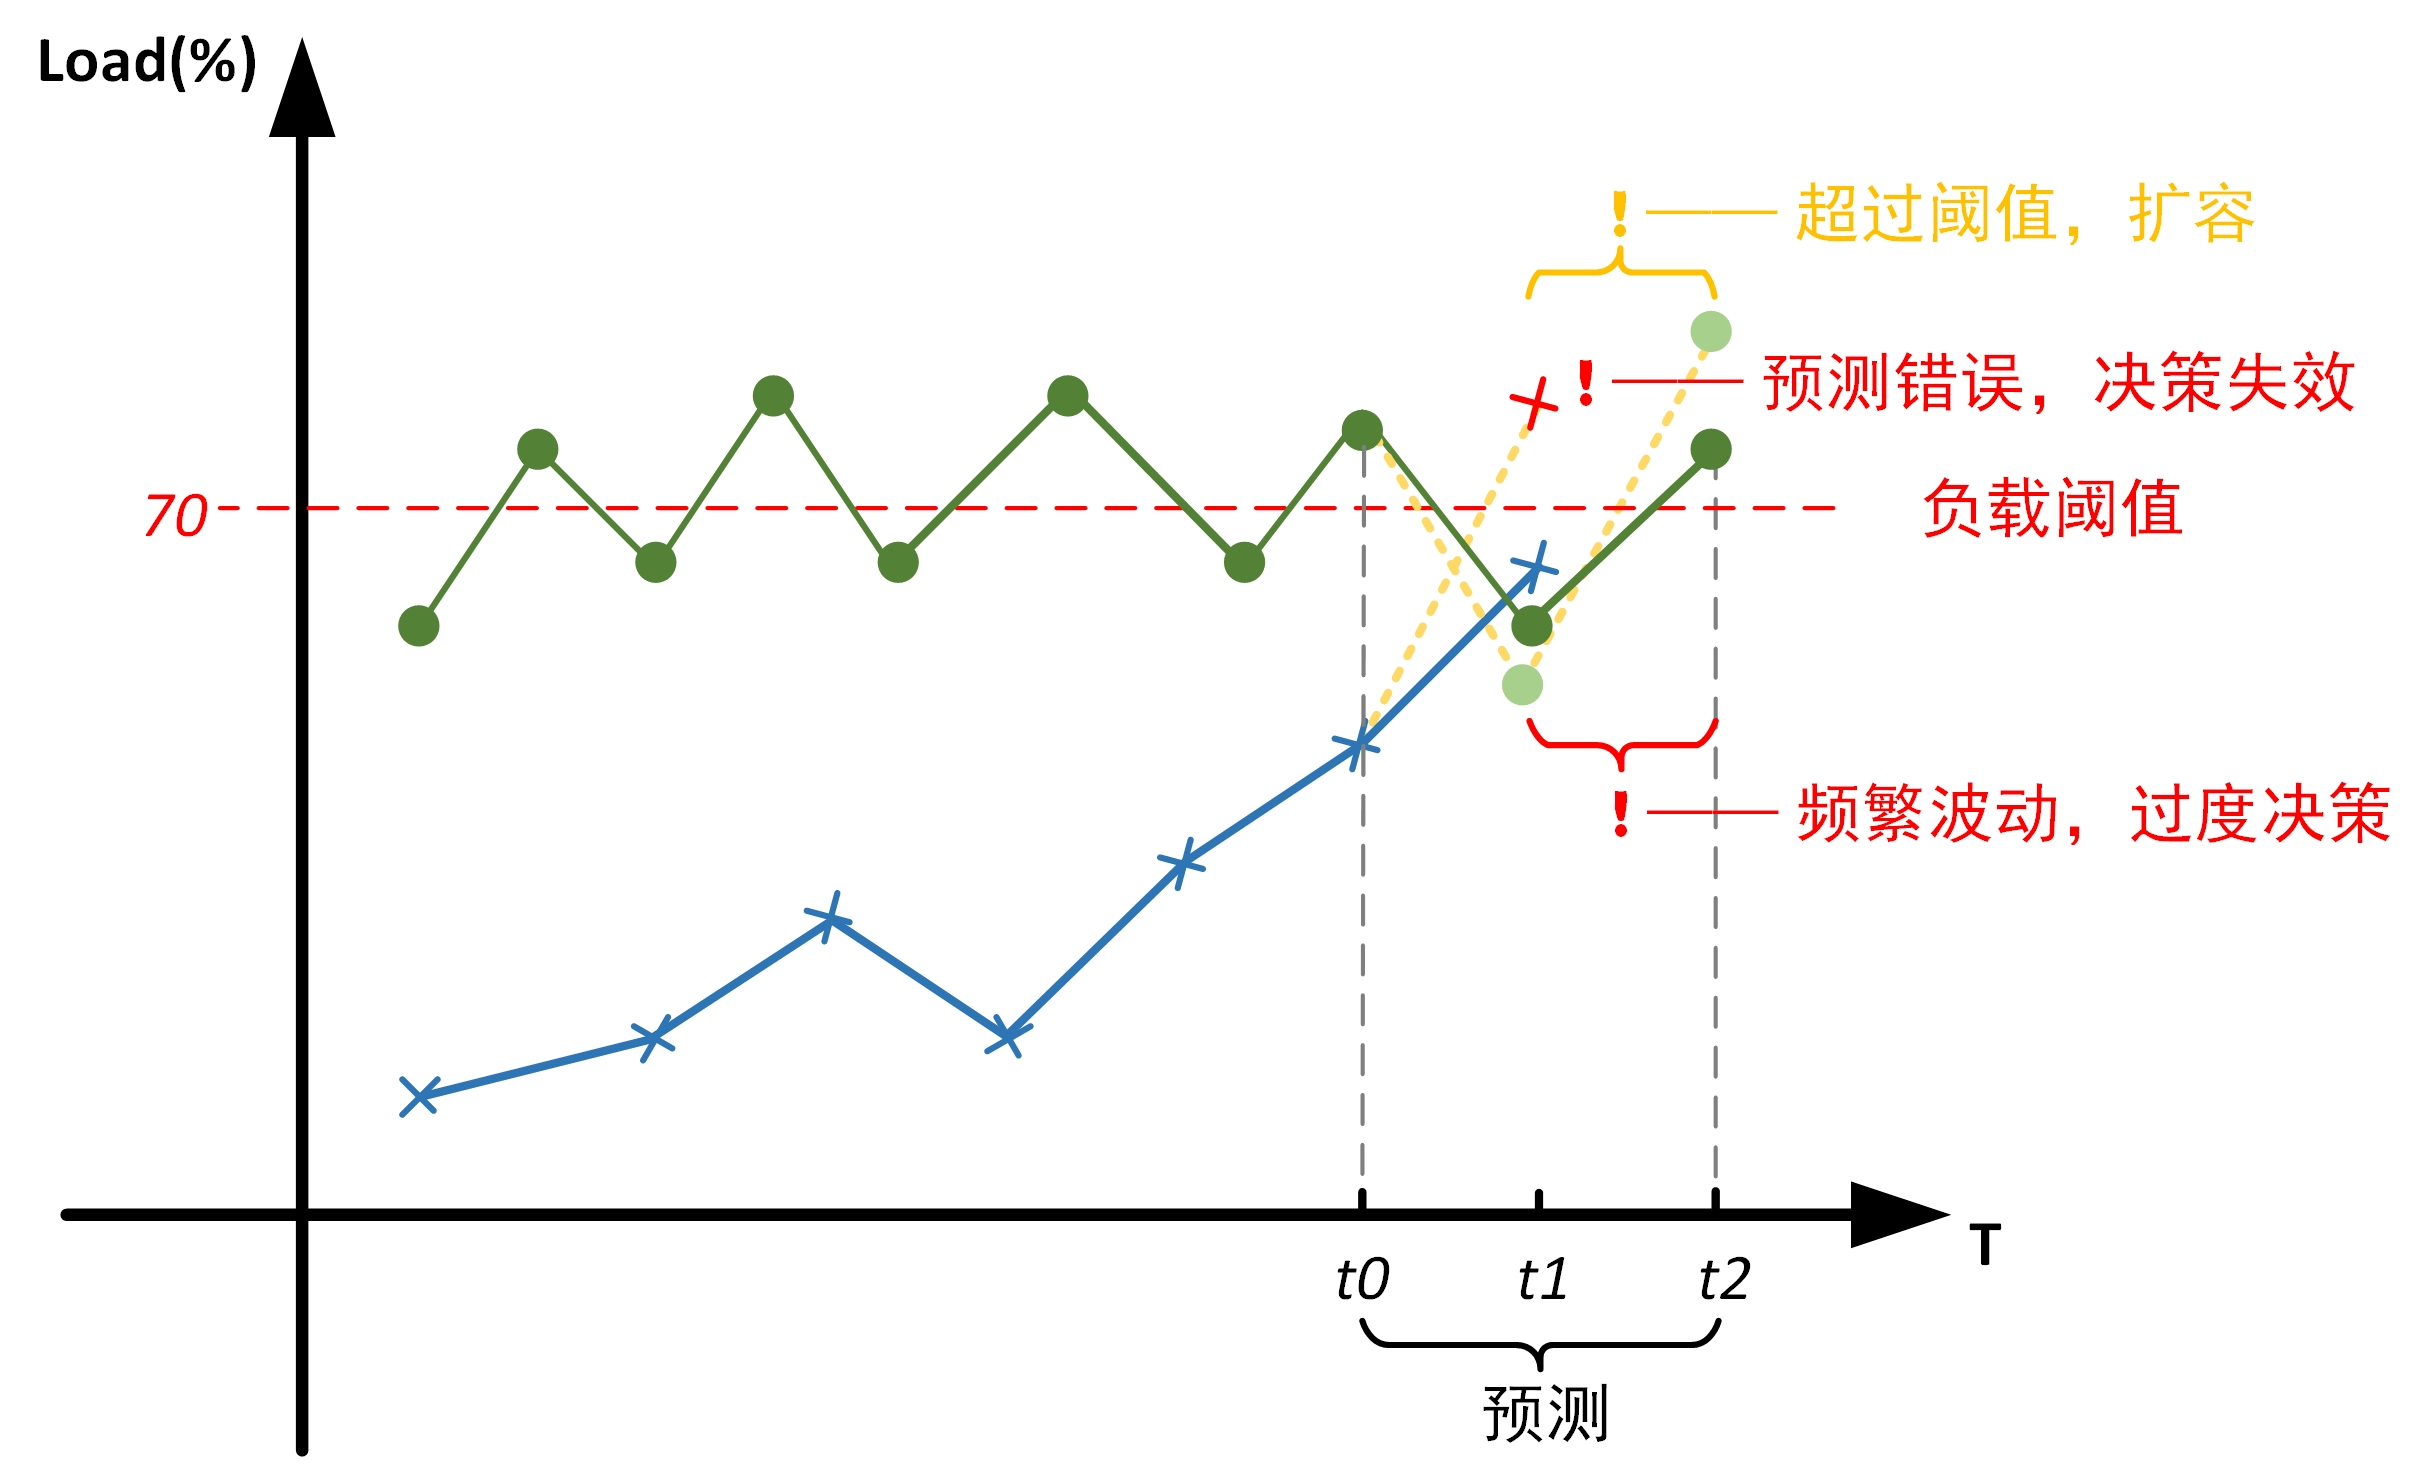
\includegraphics[scale=0.4]{figures/fig4_single_model.jpg}
\caption{单值预测模型}
\end{figure}
\end{column}
\end{columns}
}
\vspace*{-4.54cm}
\visible<2>{
\begin{columns}
\begin{column}{0.6\textwidth}
    \begin{table}[hftb]
    \centering
    \resizebox{\textwidth}{!}{%
        \begin{tabular}{ccl}
            \toprule
            \textbf{类型} & \textbf{模型名称} & \textbf{简述}\\
            \midrule
            概率论模型 & 贝叶斯模型 & 根据样本分布假设和统计学特征扩展区间\\
            \midrule
            \multirow{4}{*}{机器学习模型} & 线性回归 & \multirow{4}{*}{先拟合单值再根据分布假设构建区间}\\
            ~ & SVM & \\
            ~ & CART & \\
            ~ & 随机森林 & \\
            \bottomrule
        \end{tabular}
    }
    \caption{区间预测模型}
    \end{table}
\end{column}
\begin{column}{0.3\textwidth}
\end{column}
\end{columns}
}
\end{frame}

\subsection{容器调度}

\begin{frame}
\frametitle{研究动机}
\framesubtitle{容器调度}
\end{frame}

\end{document}
